
\documentclass{beamer}
\usetheme{Boadilla}

\usepackage[T2A]{fontenc}			% кодировка
\usepackage[utf8]{inputenc}			% кодировка исходного текста
\usepackage[english,russian]{babel}	% локализация и переносы

\usepackage{amsmath,amssymb}
\usepackage{autonum}
\usepackage{wrapfig}

\usepackage{array}
\newcommand{\PreserveBackslash}[1]{\let\temp=\\#1\let\\=\temp}
\newcolumntype{C}[1]{>{\PreserveBackslash\centering}p{#1}}


%\usepackage[font=scriptsize,format=plain,labelfont=bf,up,textfont=it,up]{caption}
%\setbeamertemplate{caption}[numbered]
\usepackage[labelformat=empty]{caption}
%\usetheme{Dresden}
%\usefonttheme[onlymath]{serif}
%\usecolortheme{dove}
\graphicspath{{./images/}}
\setbeamertemplate{navigation symbols}{}
\usepackage{ragged2e}
\newcommand{\jj}{\righthyphenmin=20 \justifying}


\begin{document}

\begin{frame}
	\begin{center}\tiny
		Федеральное государственное бюджетное образовательное учреждение высшего образования \\ «Московский государственный технический университет имени Н.Э. Баумана (национальный исследовательский университет)» (МГТУ им. Н.Э. Баумана)\\
		Факультет «Фундаментальные науки»\\
		Кафедра «Физика»\\
    \end{center}

	\begin{center}
		
\includegraphics[width=0.15\linewidth]{emb}
	\end{center}

	\begin{center}
\tiny \textbf{КВАЛИФИКАЦИОННАЯ РАБОТА МАГИСТРА ТЕХНИКА И ТЕХНОЛОГИИ \\ ПО НАПРАВЛЕНИЮ 14040000.62 «ТЕХНИЧЕСКАЯ ФИЗИКА»}\\
\vspace{0.2cm}
\tiny \textbf{НА ТЕМУ:}\\
\vspace{0.1cm}
\tiny \textbf{<<РОЛЬ ДАЛЬНОДЕЙСТВИЯ ПРИТЯЖЕНИЯ \\ В НУКЛЕАЦИИ И В КОЛЛЕКТИВНЫХ ВОЗБУЖДЕНИЯХ>>}\\
\end{center}

\vspace{0.3cm}

\begin{columns}
\begin{column}{0.50\textwidth}
\begin{center}
\tiny Выполнил: \\
\vspace{0.1cm}
\tiny \textbf{Дмитрюк Никита Александрович}\\
\tiny студент группы ФН4-41M \\
\vspace{0.2cm}
\end{center}
\end{column}


\begin{column}{0.50\textwidth}
\begin{center}
\tiny Научный руководитель:\\
\vspace{0.1cm}
\tiny \textbf{Юрченко Станислав Олегович} \\
\tiny д.ф.-м.н., профессор кафедры физики\\
\tiny МГТУ им. Н.Э. Баумана \\
\end{center}


\end{column}
\end{columns}


\vspace{0.5cm}
\begin{center}
\tiny Москва, $2022$
\end{center}
\end{frame}










\begin{frame}{Актуальность}
\footnotesize{

\textbf{Актуальность данной работы заключается в следующем:}
\begin{itemize}
    \item Нет точных данных о том, как потенциал взаимодействия частиц влияет на транспортные свойства вещества, в том числе температурные зависимости диффузии и подвижности.

    \item Неизвестно, существует ли корреляция между диффузией и спектрами возбуждений в жидкой фазе веществ.

    \item Неизвестно, каким образом дальнодействие притяжения влиет на скорость процесса кристаллообразования.

\end{itemize}

}
\end{frame}










\begin{frame}{Цель работы}
\footnotesize{
\textbf{Цель работы} -- установить связь дальнодействия потенциала и спектров возбуждений с транспортными свойствами жидкостей, а также его влияние на скорость нуклеации.

}
\end{frame}










\begin{frame}{Задачи работы}
\footnotesize{

\textbf{Задачами работы являются:}
\begin{itemize}
\item Расчет фазовых диаграмм обобщенного потенциала Леннарда-Джонса.
\item Расчет и анализ транспортных свойств и коллективных возбуждений на жидкостных бинодалях.
\item Адаптация метода кластеризации данных DBSCAN для МД моделирований.
\item Расчет фазовых диаграмм для 2D и 3D систем частиц, взаимодействующих посредством обобщенного нормированного потенциала Леннарда--Джонса с различными степенями притяжения.
\item Сравнение нового метода с другими алгоритмами распознавания фаз и построения фазовых диаграмм.
\item Проведение тестов на устойчивость метода к изменению средней плотности системы и параметров моделирования.
\item Применение нового метода распознавания фаз для изучения скорости нуклеации в переохлажденных системах Леннарда-Джонса с различным дальнодействием притяжения.
\end{itemize}


}
\end{frame}





\begin{frame}
\begin{center}
\vspace{5mm}
\textbf{<<ВЛИЯНИЕ ДАЛЬНОДЕЙСТВИЯ ПРИТЯЖЕНИЯ НА ТРАНСПОРТНЫЕ СВОЙСТВА ВЕЩЕСТВ И КОЛЛЕКТИВНЫЕ ВОЗБУЖДЕНИЯ>>}
\end{center}
\end{frame}












\begin{frame}{Параметры моделирований}
\footnotesize{

\begin{columns}
\begin{column}{0.5\linewidth}

\centering \textbf{LJn-m}

\begin{equation}
U_{n-m}(r)=4 \varepsilon\left[\left(\frac{\sigma}{r}\right)^{n}-\left(\frac{\sigma}{r}\right)^{m}\right]
\label{eqGenLJ}
\end{equation}
\jj где $\epsilon = 1$ и $\sigma = 1$ - магнитуда и \\ характерный масштаб отталкивания соответственно.

\vspace{0.0cm}

\begin{figure}
\centering
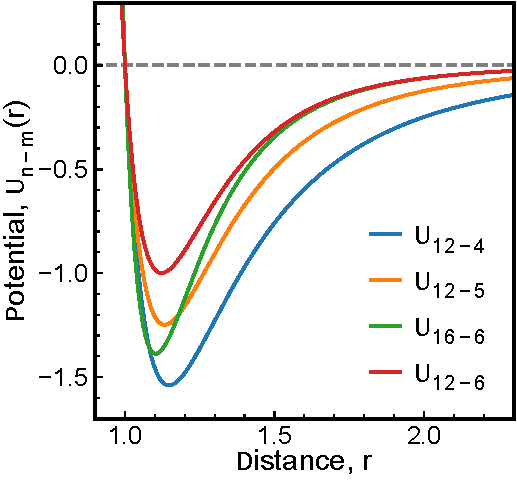
\includegraphics[width=0.8\textwidth]{LJ_no_norm.pdf}
\end{figure}

\end{column}

\begin{column}{0.5\linewidth}

\vspace{0.4cm}
\centering \textbf{Ethane}

\begin{equation}
U_{ethane}(r) = \tilde \varepsilon\left[\left(\frac{\sigma}{r}\right)^{16}-\left(\frac{\sigma}{r}\right)^{6}\right],
\label{eqEthan}
\end{equation}
\jj где $\tilde \varepsilon = 0.695$ ккал/моль; $\sigma = 3.783$\AA.

\vspace{1.0cm}

\begin{figure}
\centering
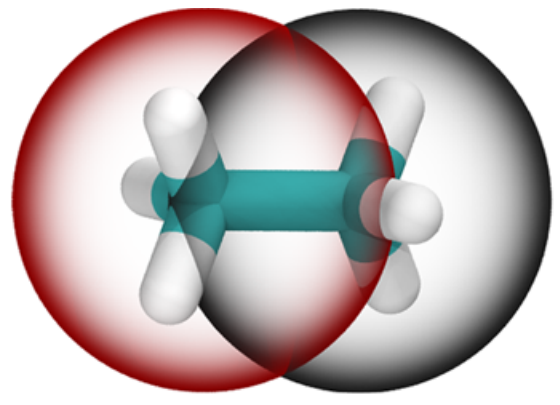
\includegraphics[width=0.7\textwidth]{ethane2.png}
\end{figure}

\vspace{0.5cm}

\end{column}
\end{columns}

}

%\vspace{0.2cm}
\tiny{J. R. Mick, et al., Journal of Chemical $\And$ Engineering Data 62, 1806 (2017).}

\end{frame}






\begin{frame}{Построение фазовых диаграмм}
\footnotesize{

% \begin{figure}
%     \centering
%      \includegraphics[width=0.6\textwidth]{Ris/MACR-Figure0.png}
% \end{figure}

% \begin{equation}
%     n(x)=\frac{n_{c}+n_{g}}{2}-\frac{n_{c}-n_{g}}{2} \tanh \left(\frac{|x|-L}{\delta}\right)
% \end{equation}
% где $L$ - половина размера области конденсированной фазы; \\
% $\delta$ - характерная толщина интерфейса.

\begin{columns}
\begin{column}{0.55\linewidth}

\vspace{0.5cm}
\begin{figure}
    \centering
    \href{run:video_flat_layer.mp4}{\includegraphics[width=\textwidth]{MACR-Figure0.png}}
    %\includegraphics[width=\textwidth]{Ris/MACR-Figure0.png}
\end{figure}


\end{column}

\begin{column}{0.48\linewidth}

\begin{equation}
    \rho(x)=\frac{\rho_{c}+\rho_{g}}{2}-\frac{\rho_{c}-\rho_{g}}{2} \tanh \left(\frac{|x|-L}{\delta}\right)
\end{equation}
\jj{где $L$ - половина размера области \\ конденсированной фазы; \\
$\delta$ - характерная толщина
интерфейса.}

\vspace{0.5cm}

\begin{table}[h!]
    \footnotesize
    \centering
    \begin{tabular}{c|c|c|c|c}
        LJ$n$-$m$ & $\rho$ & $r_c$ & $T_{\rm start}$ & $T_{\rm stop}$ \\ \hline
        LJ12-4 & 0.25 & 15.0 & 1.0 & 5.5 \\
        LJ12-5 & 0.25 & 10.0 & 0.8 & 2.4\\
        LJ12-6 & 0.35 & 8.0 & 0.5 & 1.4\\
        LJ16-6 & 0.31 & 8.0 & 0.8 & 1.6\\
    \end{tabular}

    \label{MACR-Table1}
\end{table}

\end{column}
\begin{column}{0.001\linewidth}
\end{column}

\end{columns}

}

\vspace{0.5cm}
\tiny{F. Biscay, et al., The Journal of Physical Chemistry B 112, 13885 (2008).}

\end{frame}









\begin{frame}{Построение фазовых диаграмм}
\footnotesize{
\begin{columns}
\begin{column}{0.6\linewidth}

\vspace{0.1cm}

\begin{figure}
    \centering
    \caption{\footnotesize Фазовая диаграмма системы LJ12-6.}
    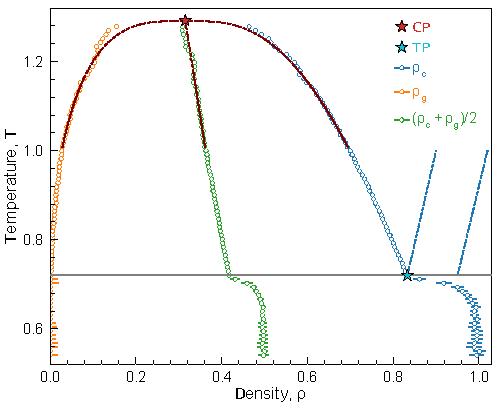
\includegraphics[width=\textwidth]{MACR-Figure-1.pdf}

\end{figure}


\end{column}

\begin{column}{0.45\linewidth}

\begin{equation}
    \rho_{c}-\rho_{g} \simeq A \tau^{\beta}, \quad \rho_{c}+\rho_{g} \simeq a \tau+2 \rho_{\mathrm{CP}},
\label{eqFitFlatLayer}
\end{equation}
\jj{где $\tau=T_{\mathrm{CP}}-T$; \\
$T_{\mathrm{CP}}$ и $\rho_{\mathrm{CP}}$ - температура и
плотность в критической точке соответственно; \\
$\beta$ - критический индекс.}

\vspace{0.5cm}

\jj $\beta = 0.5$ для LJ12-4 и $\beta = 0.325$ для других рассматриваемых потенциалов.

\end{column}
\end{columns}

}

\vspace{0.5cm}
\tiny{E. Luijten et al., Physical Review Letters 89, 025703 (2002).\\
F. Biscay, et al., The Journal of Physical Chemistry B 112, 13885 (2008).}
\end{frame}










\begin{frame}{Вычисление диффузии и спектров в жидкости}
\footnotesize{
\begin{columns}
\begin{column}{0.55\linewidth}
\begin{center}

\begin{figure}
\caption{\footnotesize Зависимость среднеквадратичного смещения частиц от времени.}
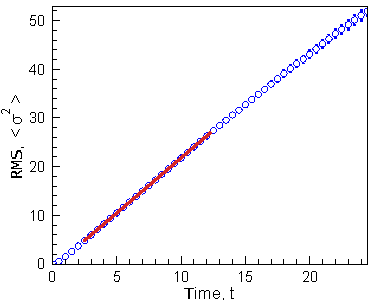
\includegraphics[width=\textwidth]{Fig_support_1.pdf}
\end{figure}
  \end{center}

\end{column}

\begin{column}{0.5\linewidth}

Cреднеквадратичное смещение частиц:
\begin{align}
    \sigma^2(t) &= \sum\limits_{\alpha = 1}^{N} (r_{\alpha}(t) - r_{\alpha}(0))^2 / N \\
    \sigma^2(t) &= 6\cdot D\cdot t
    \label{eqRMS}
\end{align}

где $D$ - коэффициент диффузии;

$\sigma$ - среднеквадратичное смещение;

$t$ - время;

$N$ - количество частиц.

\vspace{0.5cm}

Подвижность частиц $\mu$ связана с диффузией:
\begin{equation}
    \mu = \frac{D}{T}
    \label{eqMobility}
\end{equation}

\end{column}
\end{columns}


}

\end{frame}










\begin{frame}{Вычисление диффузии и спектров в жидкости}
\footnotesize{
\begin{columns}
\begin{column}{0.5\linewidth}
\begin{center}
    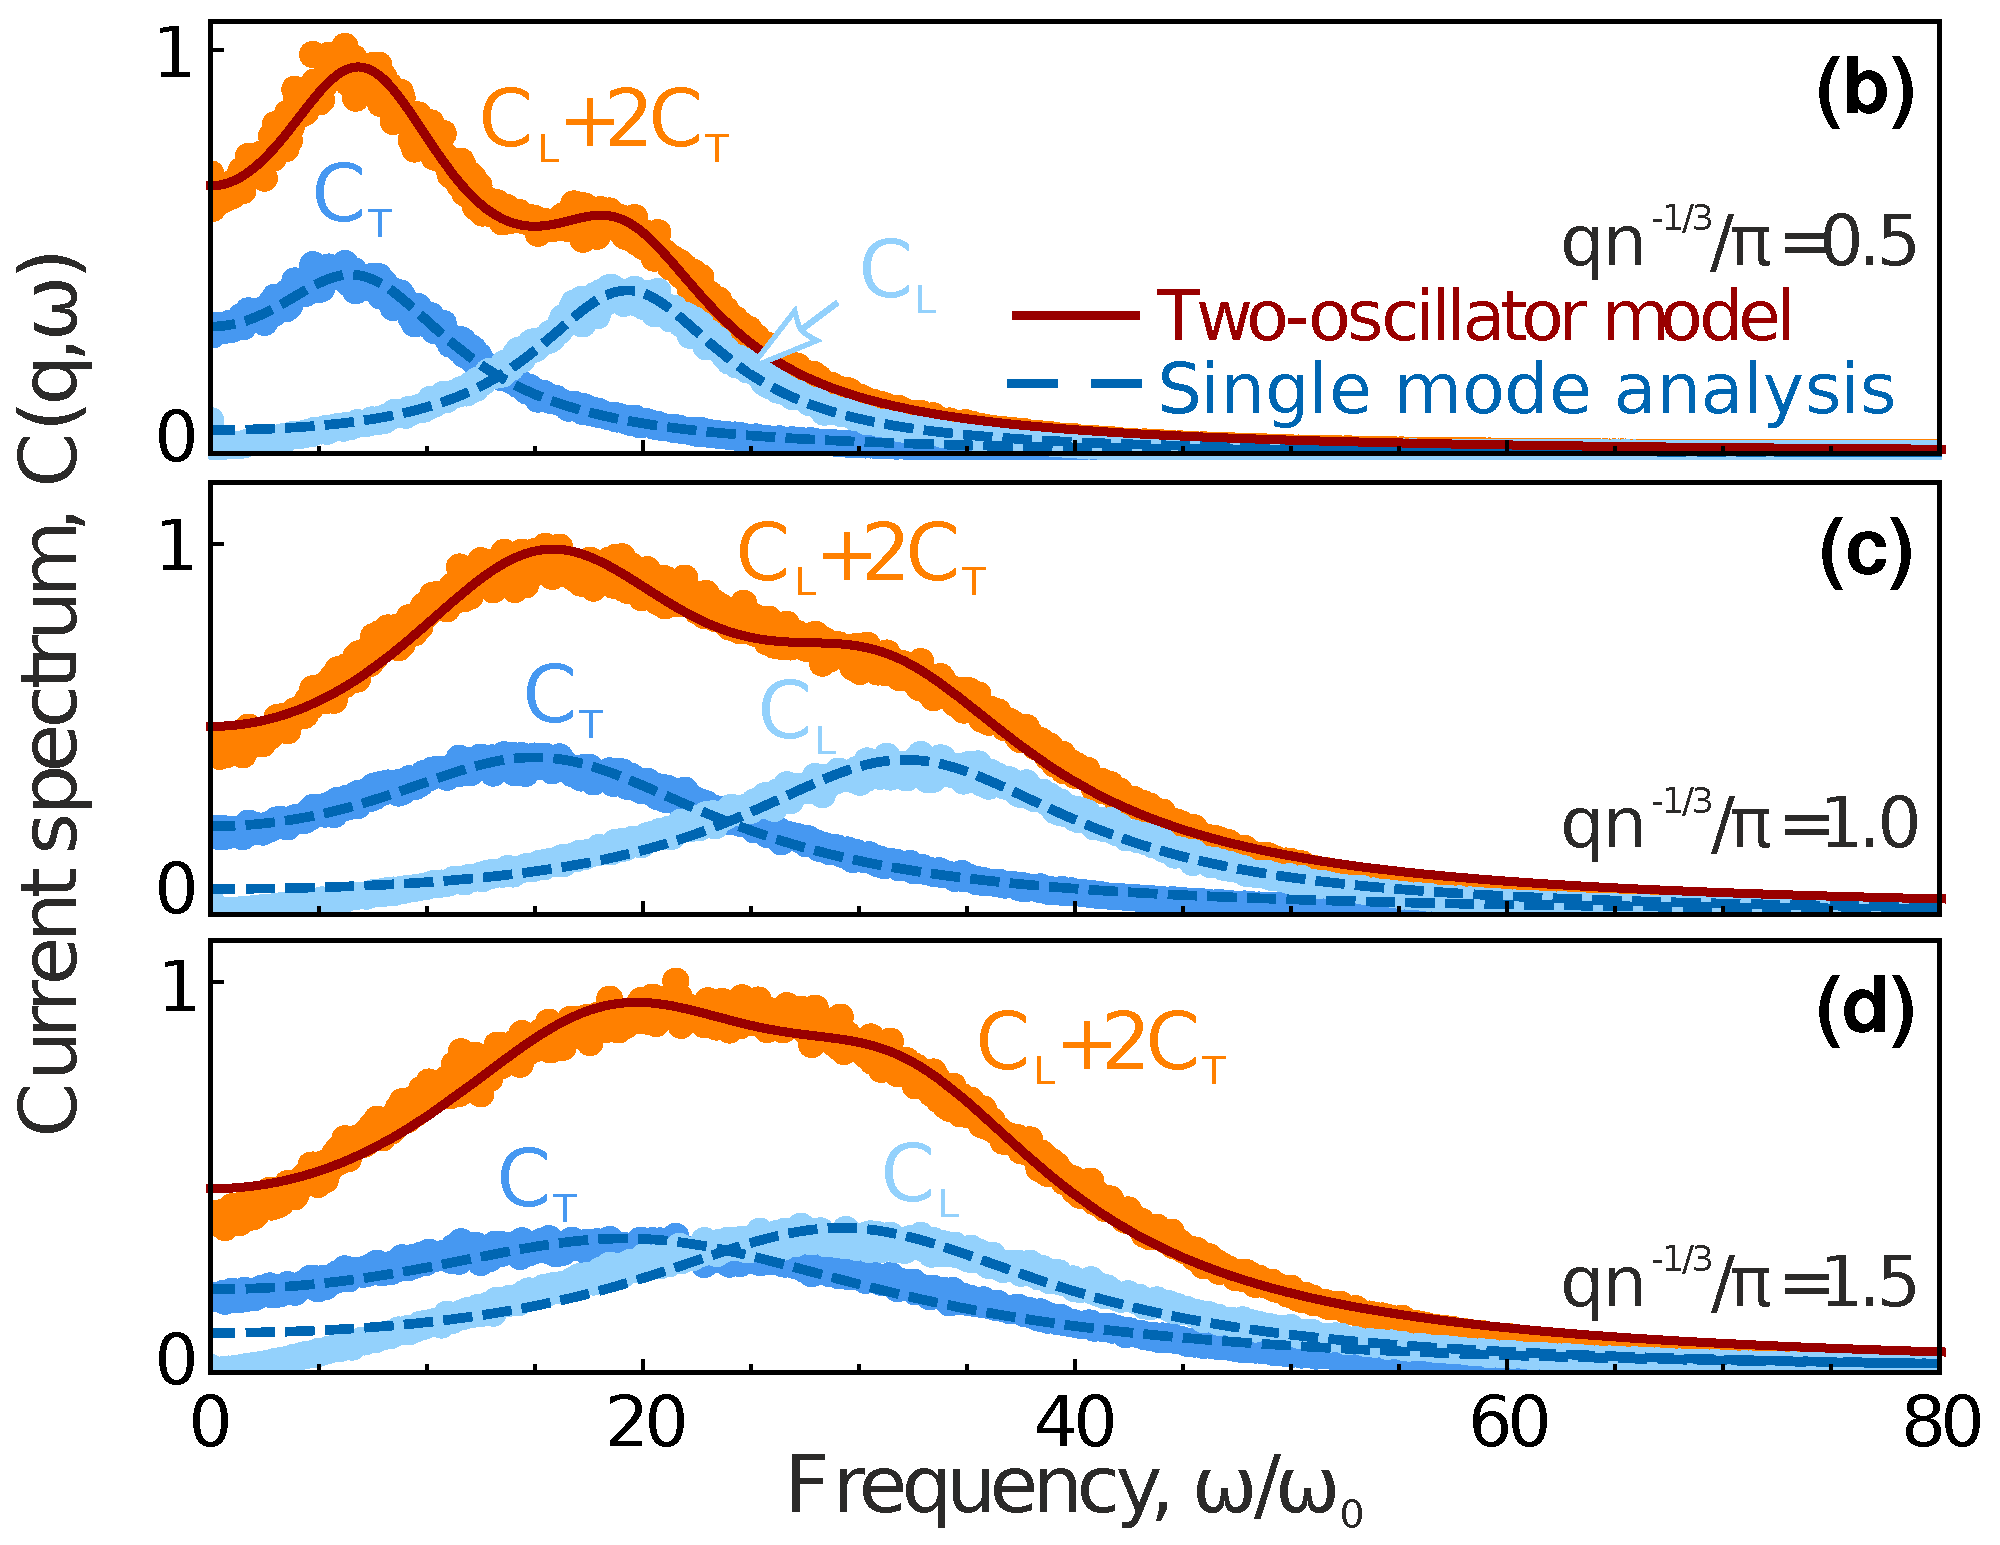
\includegraphics[width=\textwidth]{CFS-Figure1.png}
  \end{center}

\end{column}

\begin{column}{0.5\linewidth}

Спектр потока скорости:
\begin{align}
    C_{L, T}(\mathbf{q}, \omega)&=\int dt e^{i \omega t} \text{Re} \left\langle\mathbf{j}_{L, T}(\mathbf{q}, t) \mathbf{j}_{L, T}(-\mathbf{q}, 0)\right\rangle \\
    \text{где} \quad \mathbf{j}(\mathbf{q}, t)&=N^{-1} \sum_{s} \mathbf{v}_{s}(t) \exp \left(i \mathbf{q} \mathbf{r}_{s}(t)\right)
\end{align}

\end{column}
\end{columns}


\vspace{0.5cm}

Полный спектр потока скорости $C(q, \omega) = C_L(q, \omega) + (D-1)C_T(q, \omega)$:
\begin{equation}
    \begin{aligned}
    C(q, \omega) & \propto \frac{\Gamma_{L}}{\left(\omega-\omega_{L}\right)^{2}+\Gamma_{L}^{2}}+\frac{\Gamma_{L}}{\left(\omega+\omega_{L}\right)^{2}+\Gamma_{L}^{2}}+\frac{(D-1) \Gamma_{T}}{\left(\omega-\omega_{T}\right)^{2}+\Gamma_{T}^{2}}+\frac{(D-1) \Gamma_{T}}{\left(\omega+\omega_{T}\right)^{2}+\Gamma_{T}^{2}}
\end{aligned}
\label{eq5}
\end{equation}

}

\vspace{1.0cm}
\tiny{N.P. Kryuchkov, et al., Scientific Reports 9, 10483 (2019). \\
S.A. Khrapak, et al., The Journal of Chemical Physics 149, 134114 (2018).}

\end{frame}












\begin{frame}{Результаты вычисления фазовых диаграмм и подвижности}
\footnotesize{
\begin{figure}
    \centering
    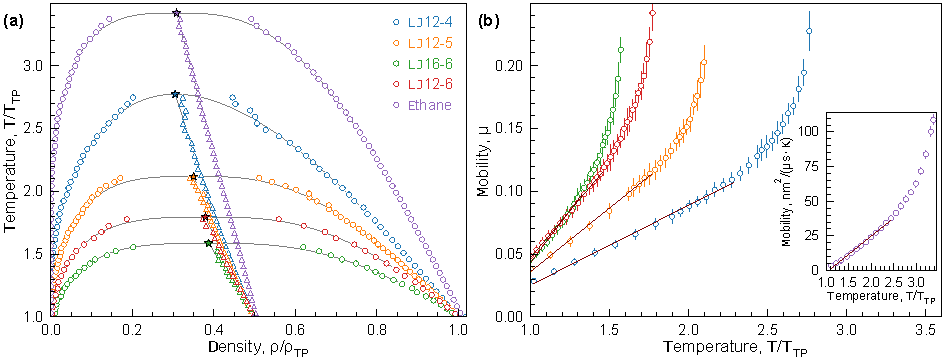
\includegraphics[width=\textwidth]{MACR-Figure3}
    \caption{\footnotesize{\textbf{(a) Фазовые диаграммы рассматриваемых потенциалов:} фазовые диаграммы рассчитаные плоским слоем.\\
 \textbf{(b) Температурная зависимость подвижности частиц:} подвижность частиц рассчитанная на бинодали жидкость -- газ.}}
\end{figure}

}

\tiny{Influence of Long-Range Potential Action on Mobility on a Liquid Binodal / Nikita A. Dmitryuk, Lucia A. Mistryukova, Nikita P. Kryuchkov, Sergey A. Khrapak, Stanislav O. Yurchenko. // \textit{The Journal of Chemical Physics}}

\end{frame}








\begin{frame}{Результаты совместного анализа}
\scriptsize{

\begin{figure}
\centering
 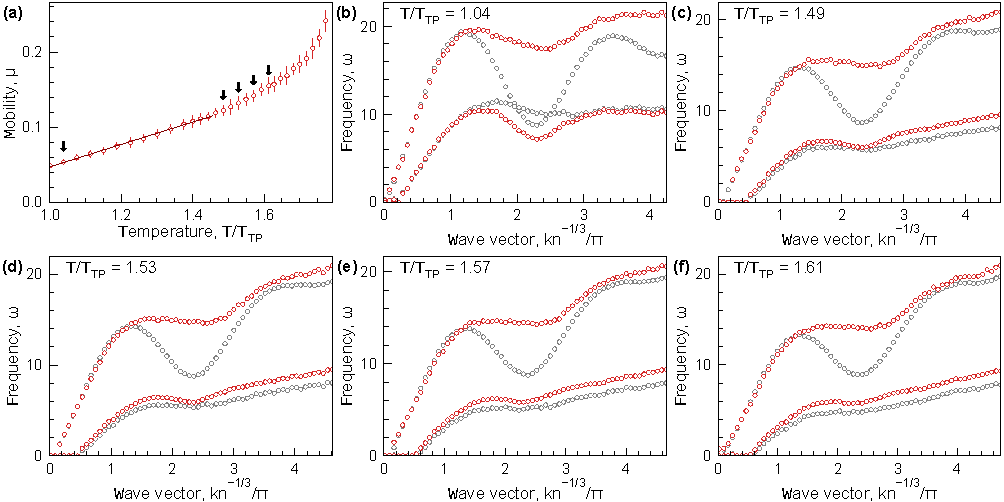
\includegraphics[width=0.95\textwidth]{MACR-Figure4}
 \caption{\scriptsize{\textbf{(a) Температурная зависимость подвижности потенциала LJ12-6:} точки, в который были рассчитаны спектры указаны черными стрелками.\\
 \textbf{(b) - (f) Спектры потенциала LJ12-6:} Красным цветом показаны спектры, рассчитанные совместным анализом мод.}}
\label{Figure4}
\end{figure}

}

\tiny{Influence of Long-Range Potential Action on Mobility on a Liquid Binodal / Nikita A. Dmitryuk, Lucia A. Mistryukova, Nikita P. Kryuchkov, Sergey A. Khrapak, Stanislav O. Yurchenko. // \textit{The Journal of Chemical Physics}}

\end{frame}








\begin{frame}{Результаты совместного анализа}
\footnotesize{

\begin{figure}
\centering
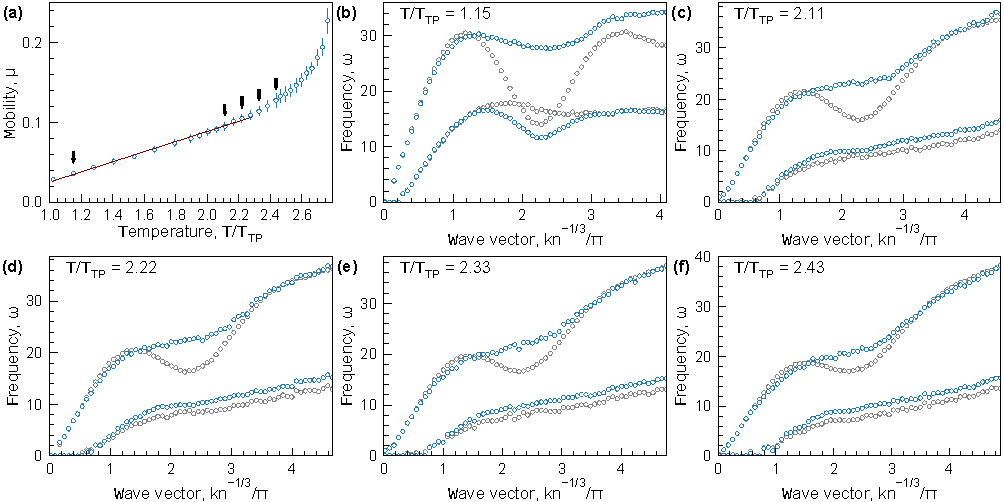
\includegraphics[width=\textwidth]{MACR-Figure5}
\caption{\footnotesize \textbf{Аналогичные графики для потенциала LJ12-4}}
\label{Figure4}
\end{figure}

}

\tiny{Influence of Long-Range Potential Action on Mobility on a Liquid Binodal / Nikita A. Dmitryuk, Lucia A. Mistryukova, Nikita P. Kryuchkov, Sergey A. Khrapak, Stanislav O. Yurchenko. // \textit{The Journal of Chemical Physics}}
\end{frame}





\begin{frame}{Результаты совместного анализа}
\footnotesize{

\begin{figure}
\centering
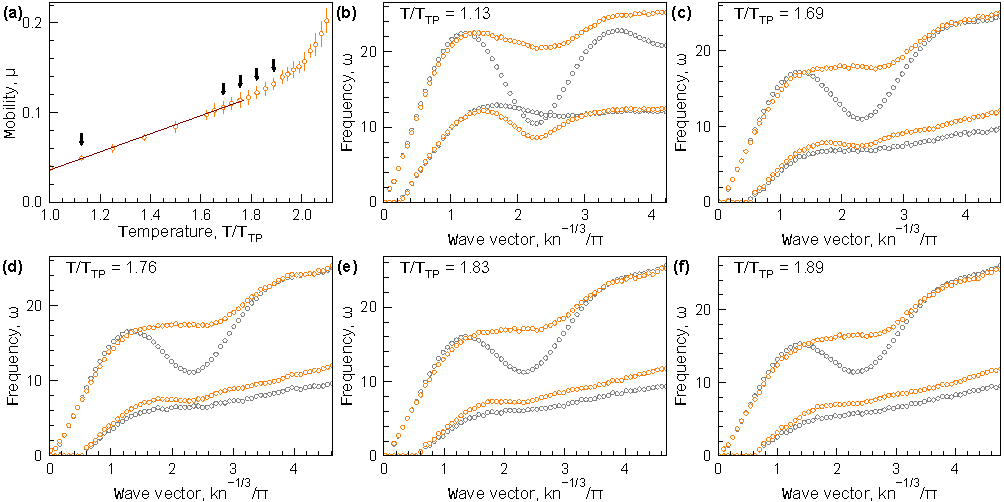
\includegraphics[width=\textwidth]{MACR-Figure6}
\caption{\footnotesize \textbf{Аналогичные графики для потенциала LJ12-5}}
\label{Figure4}
\end{figure}

}

\tiny{Influence of Long-Range Potential Action on Mobility on a Liquid Binodal / Nikita A. Dmitryuk, Lucia A. Mistryukova, Nikita P. Kryuchkov, Sergey A. Khrapak, Stanislav O. Yurchenko. // \textit{The Journal of Chemical Physics}}
\end{frame}




\begin{frame}{Результаты совместного анализа}
\footnotesize{

\begin{figure}
\centering
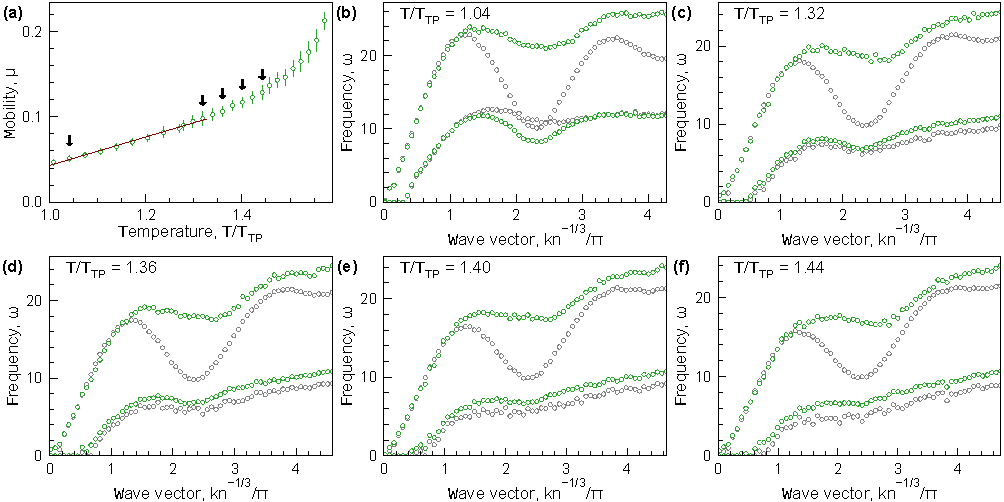
\includegraphics[width=\textwidth]{MACR-Figure7}
\caption{\footnotesize \textbf{Аналогичные графики для потенциала LJ16-6}}
\label{Figure4}
\end{figure}

}

\tiny{Influence of Long-Range Potential Action on Mobility on a Liquid Binodal / Nikita A. Dmitryuk, Lucia A. Mistryukova, Nikita P. Kryuchkov, Sergey A. Khrapak, Stanislav O. Yurchenko. // \textit{The Journal of Chemical Physics}}
\end{frame}





\begin{frame}{Выводы главы}
\footnotesize{
\begin{itemize}

    \item Обнаружено, что подвижность имеет линейную зависимость в широком диапазоне температур на конденсированной бинодали.

    \item Установлено, что при увеличении дальнодействия потенциала увеличивается отношение температур критической к тройной точки. Кроме того, при этом уменьшается наклон температурной зависимости подвижности.

    \item Продемонстрировано, что отклонение подвижности от линейной зависимости при высоких температурах коррелирует с переходом спектров возбуждений от осцилирующего к монотонному виду.

    \item Исследование подвижности на бинодали жидкость-газ для систем с различным дальнодействием притяжением поддержано грантом Российского научного фонда No 20-12-00356. Материалы данной работы готовятся к публикации <<Influence of Long-Range Potential Action on Mobility on a Liquid Binodal / Nikita A. Dmitryuk, Lucia A. Mistryukova, Nikita P. Kryuchkov, Sergey A. Khrapak, Stanislav O. Yurchenko. // \textit{The Journal of Chemical Physics}>>.
\end{itemize}

}
\end{frame}









\begin{frame}
\begin{center}
\vspace{5mm}
\textbf{<<ВЛИЯНИЕ ДАЛЬНОДЕЙСТВИЯ ПРИТЯЖЕНИЯ НА ФАЗОВЫЕ ДИАГРАММЫ И СКОРОСТЬ НУКЛЕАЦИИ>>}
\end{center}
\end{frame}








\begin{frame}{Алгоритмы кластеризации}
\footnotesize{

\begin{figure}[!t]
\begin{center}
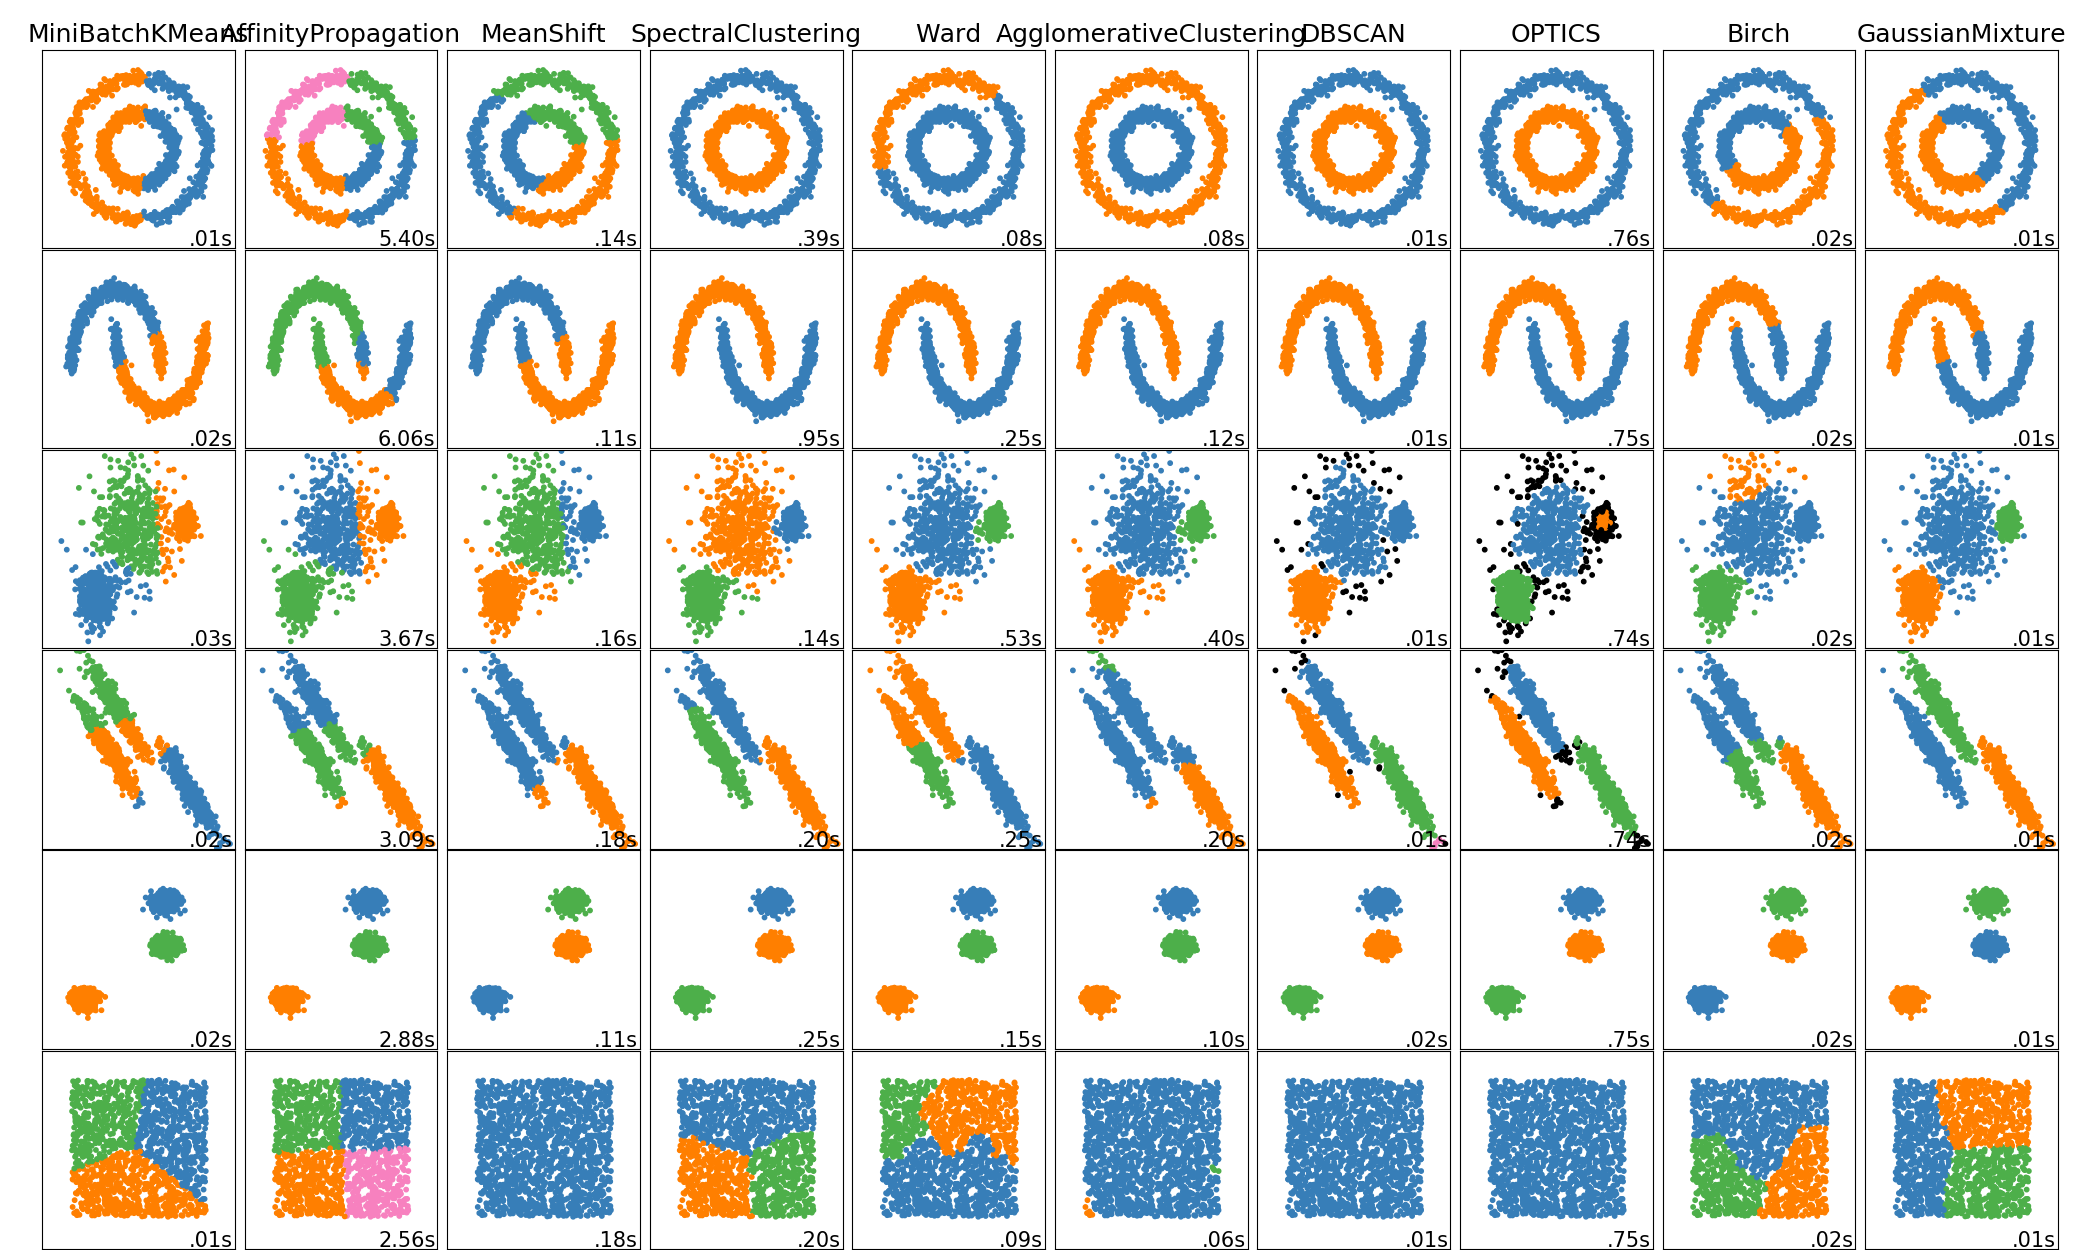
\includegraphics[width=0.85\textwidth]{Intersect.png}
\caption{Алгоритм DBSCAN применяется для кластеризации данных в которых присутствует большое количество шумов и кластеры имеют одинаковую плотность.}
\label{sravnenie}
\end{center}
\end{figure}

}

\end{frame}



\begin{frame}{Принцип работы DBSCAN}
\footnotesize{

\begin{figure}[!t]
    \centering
    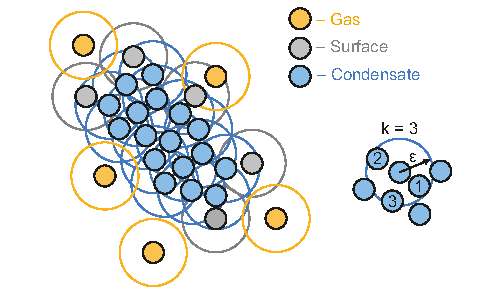
\includegraphics[width=0.9\linewidth]{kepsilon.pdf}
    \caption{Принцип работы алгоритма кластеризации DBSCAN для случая $k = 3$.}
    \label{kepsilon}
\end{figure}
}

\end{frame}




\begin{frame}{Оптимальный выбор параметра $\varepsilon$}
\footnotesize{


\begin{figure}[!t]
    \centering
    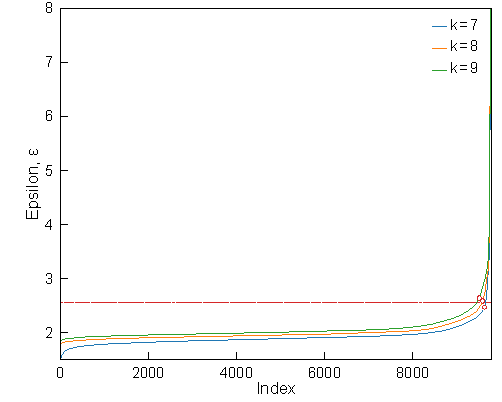
\includegraphics[width=0.7\linewidth]{Figure0.pdf}
    \caption{Выбор оптимального параметра $\varepsilon$. Красным цветом указаны точки для различных значений параметра $k$, наиболее удаленные от линии, соединяющей начало и конец кривой расстояний.}
    \label{epsilon_k}
\end{figure}
}

\end{frame}





\begin{frame}{Пример распознавания частиц в 2D системе LJ12-6.}
\footnotesize{


\begin{figure}[!t]
    \centering
    \includegraphics[width=0.8\linewidth]{PRIMe-FIgure104.pdf}
    \caption{(a) классификация частиц на конденсат и газ. \\
    (b) выделение частиц поверхности, по условию принадлежности к конденсату и не к основным частицам. \\
    (с) пример выделения регулярной поверхности, охватывающей все частицы кластера.}
    \label{DBSCAN-Illustr}
\end{figure}

}

\end{frame}




\begin{frame}{Распознавание фаз методом DBSCAN в 3D системе LJ12-6}
\footnotesize{


\begin{figure}[!t]
    \centering
    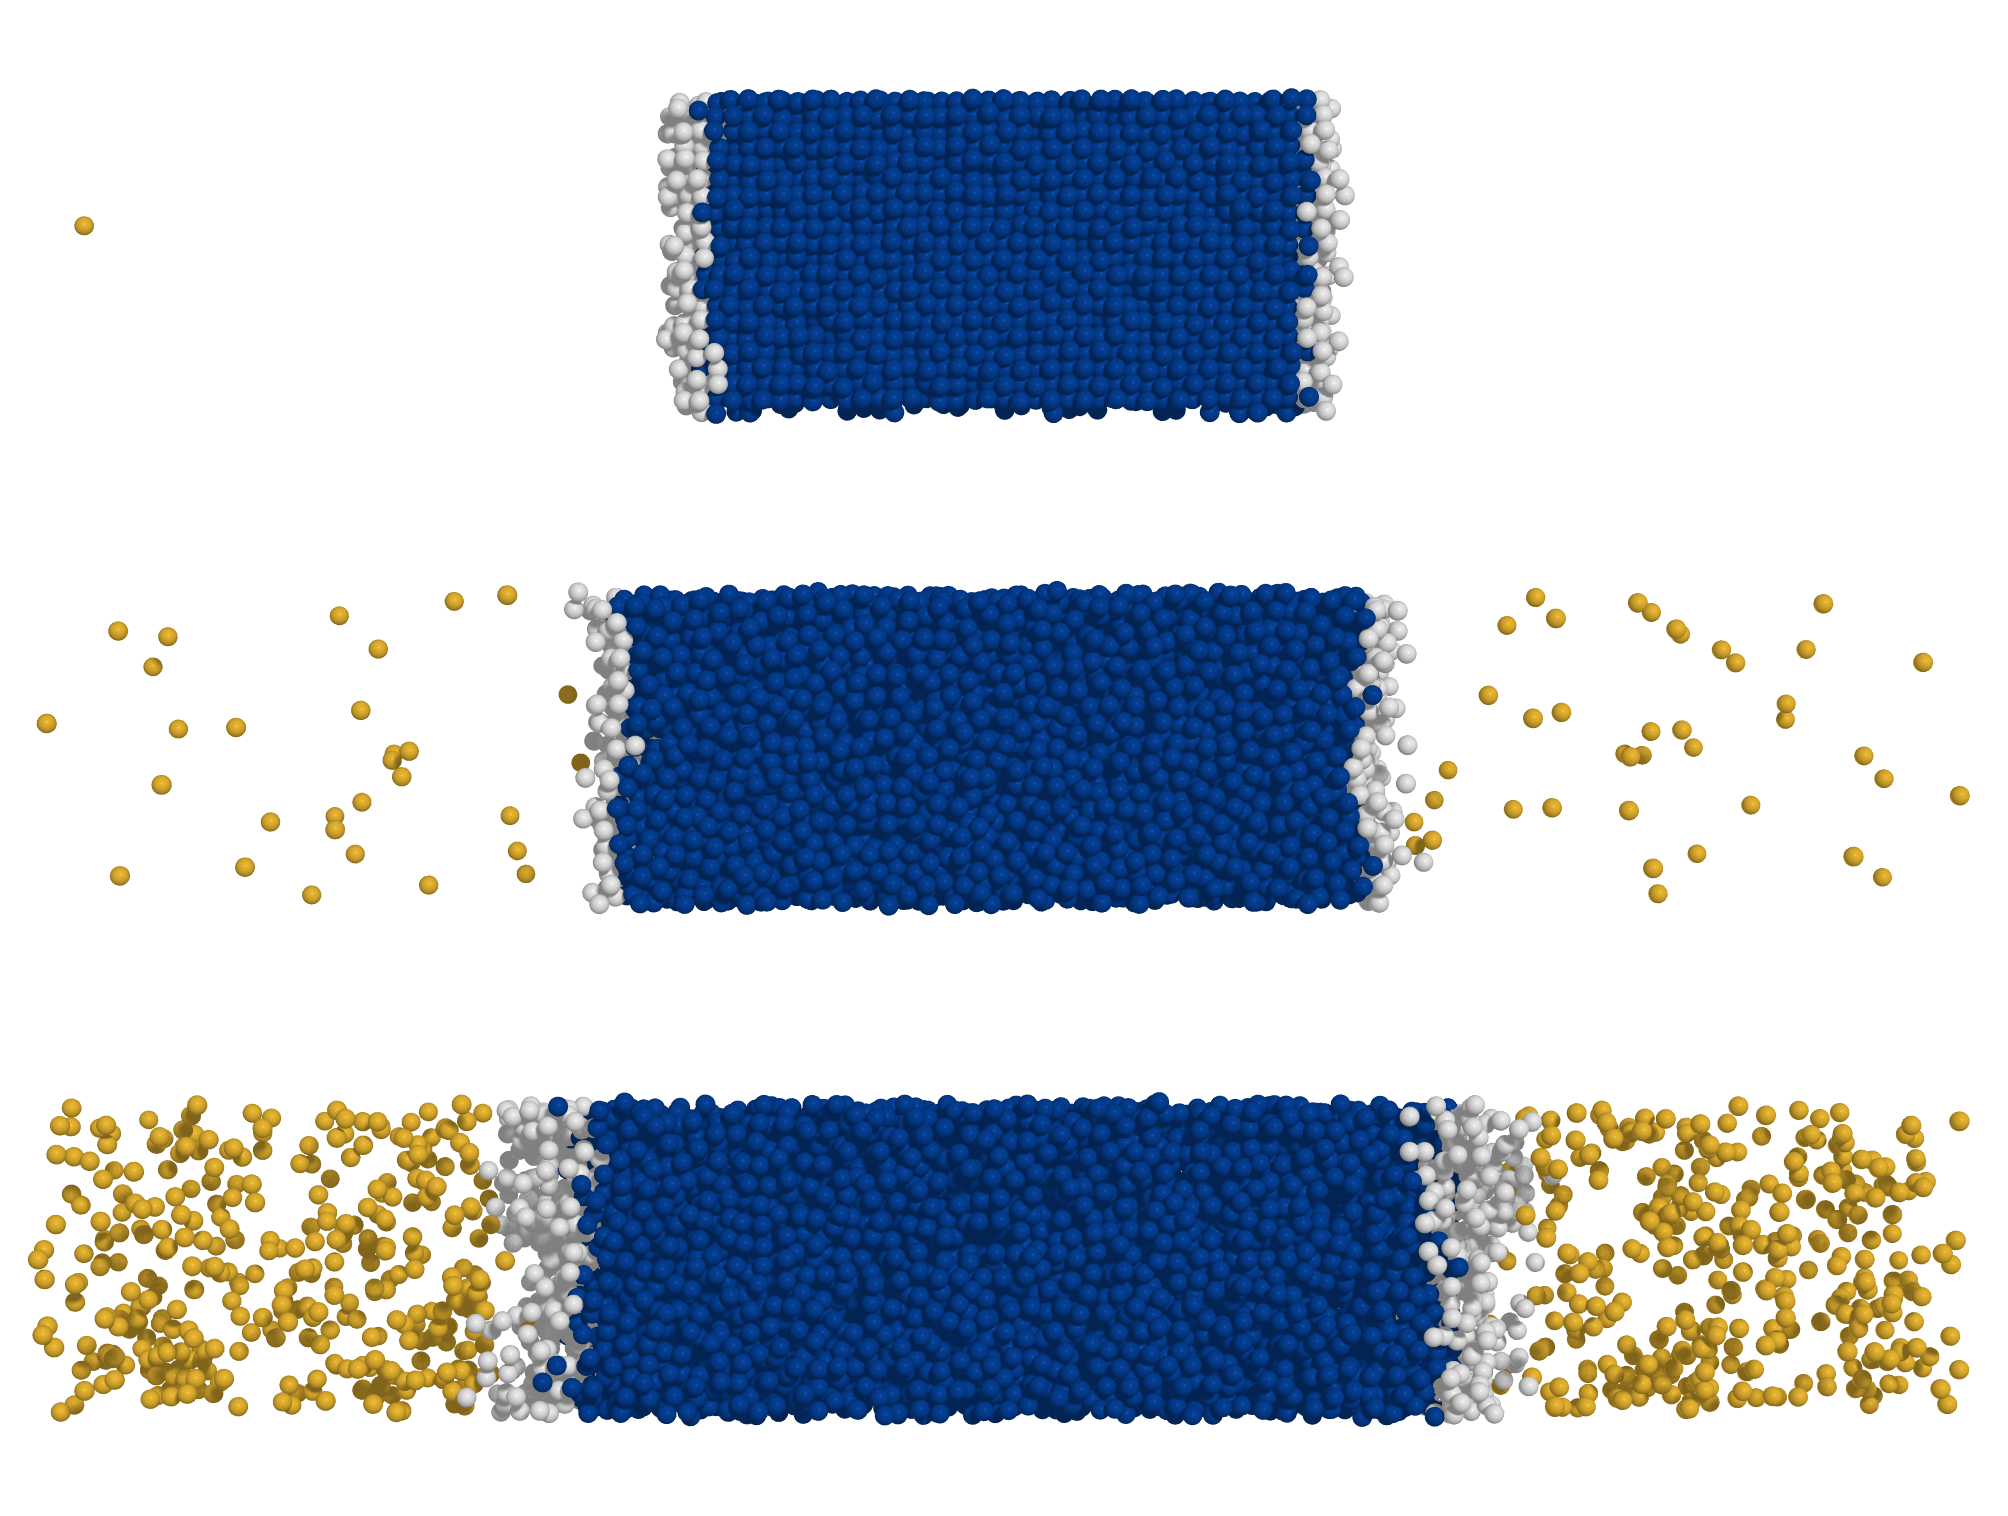
\includegraphics[width=0.8\linewidth]{PRIMe-Figure101.png}
    \label{D3_flat_layer}
\end{figure}


}

\end{frame}





\begin{frame}{Распознавание фаз методом DBSCAN в 3D системе LJ12-6}
\footnotesize{
\begin{figure}[!t]
    \centering
    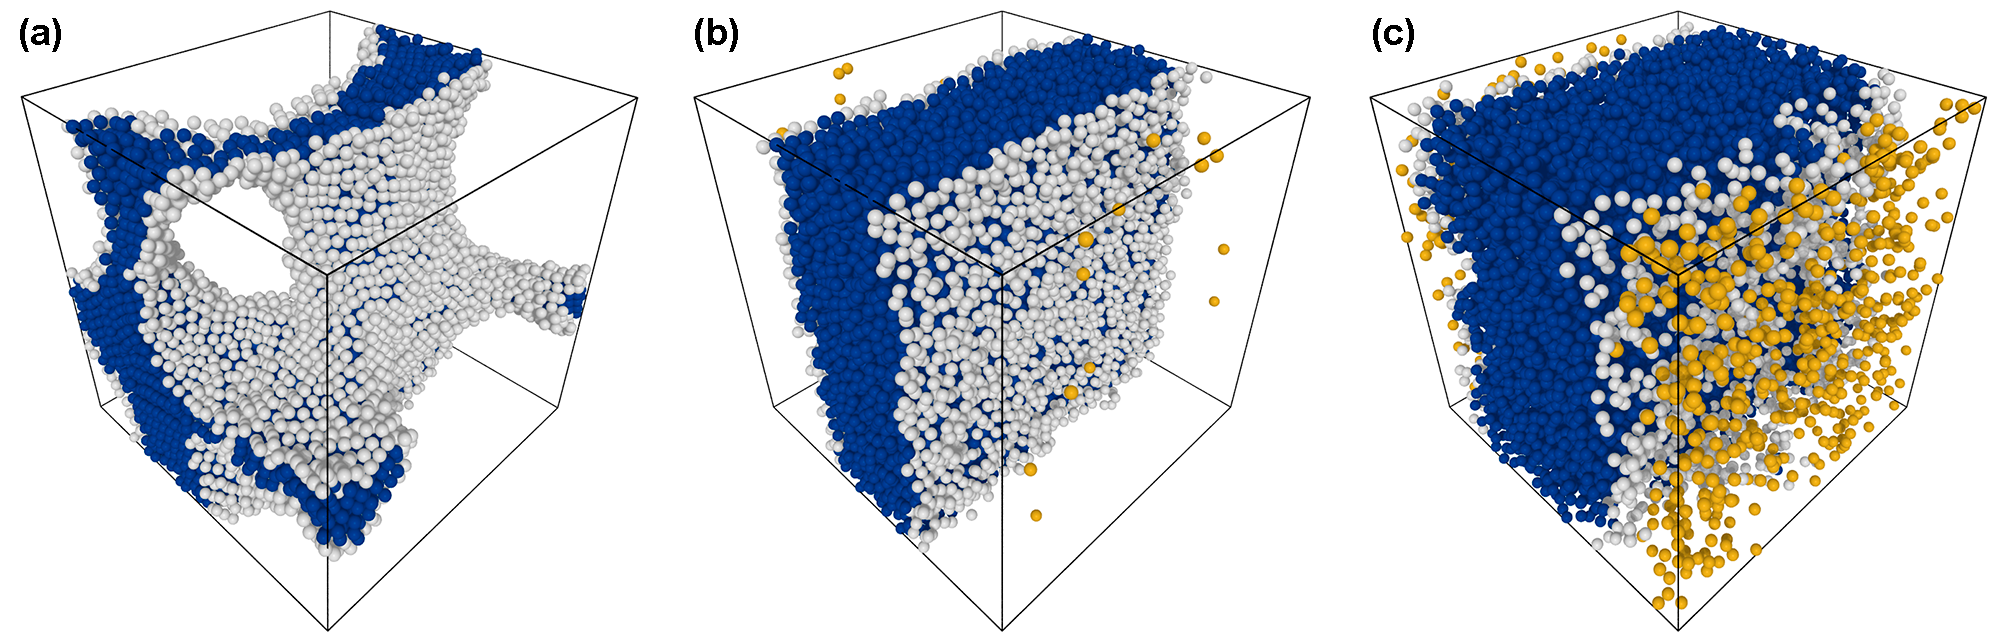
\includegraphics[width=\linewidth]{PRIMe-Figure103.png}
    \caption{(a) кластер произвольной формы при температуре ниже тройной точки. \\
    (b) система в состоянии жидкость + газ. \\
    (с) система вблизи критической точки.}
    \label{D3_free_conf}
\end{figure}
}

\end{frame}








\begin{frame}{Тесты на устойчивость метода}
\footnotesize{
\begin{figure}[!t]
    \centering
    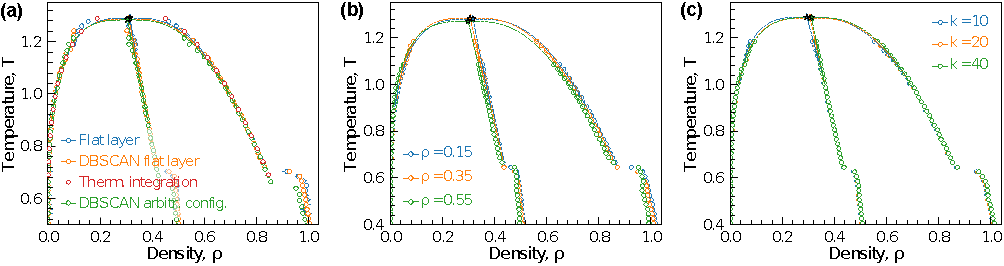
\includegraphics[width=\linewidth]{Figure10.pdf}
    \caption{\textbf{(a)} Сравнение различных методов построения фазовых диаграмм. Красным отмечен самый точный метод - термодинамическое интегрирование.\\
             \textbf{(b)} Тест на влияние средней плотности на фазовую диаграмму системы LJ12-6 в трехмерии.\\
             \textbf{(c)} Тест на влияние начального параметра $k$ на фазовую диаграмму системы LJ12-6 в трехмерии.}
    \label{tests}
\end{figure}
}

\end{frame}






\begin{frame}{Скорость нуклеации в переохлажденных системах}
\footnotesize{

\begin{equation}
U_{nm}(r)=\frac{\varepsilon}{n-m}\left(\frac{m}{r^n}-\frac{n}{r^m}\right) \label{NMP-eq1}
\end{equation}

\begin{figure}[!t]
	 \centering
	 \includegraphics[width=\linewidth]{otchet.pdf}
	 \caption{Процесс зарождения и роста кластеров в переохлажденной системе частиц взаимодействующих посредством потенциала Леннарда-Джонса.}
	 \label{otchet}
\end{figure}

}

\end{frame}





\begin{frame}{Скорость нуклеации в переохлажденных системах}
\footnotesize{
\begin{figure}[!t]
    \centering
    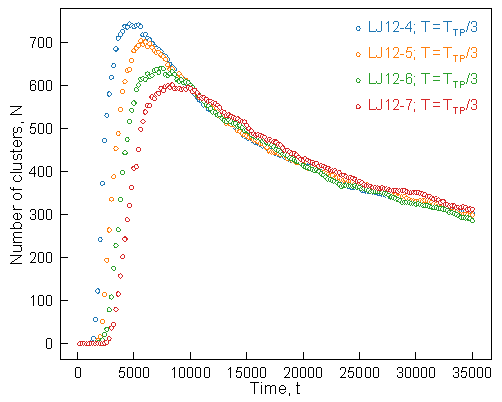
\includegraphics[width=0.7\linewidth]{countCluster.pdf}
    \caption{Зависимость количества кластеров от времени.}
    \label{countCluster}
\end{figure}
}

\end{frame}






\begin{frame}{Скорость нуклеации в переохлажденных системах}
\footnotesize{
\begin{figure}[!t]
    \centering
    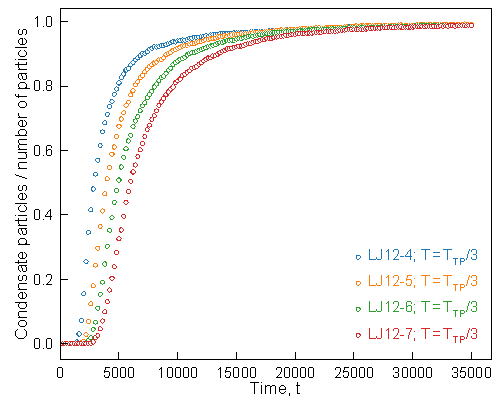
\includegraphics[width=0.7\linewidth]{countParticles.pdf}
    \caption{Зависимость доли частиц, находящихся в конденсированном состоянии от времени для различных потенциалов.}
    \label{countParticles}
\end{figure}
}

\end{frame}







\begin{frame}{Скорость нуклеации в переохлажденных системах}
\footnotesize{
\begin{figure}[!t]
    \centering
    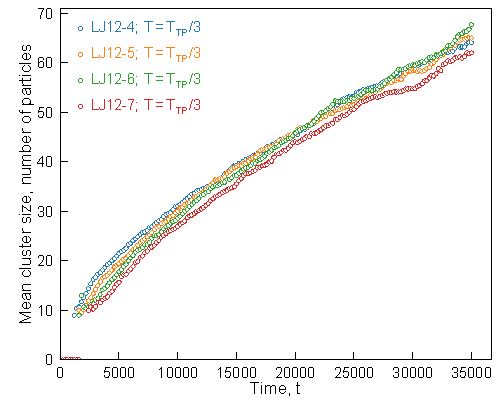
\includegraphics[width=0.7\linewidth]{meanParticles.pdf}
    \caption{Зависимость среднего размера кластера от времени для систем с различным дальнодействием потенциала.}
    \label{meanParticles}
\end{figure}
}

\end{frame}









\begin{frame}{Выводы главы}
\footnotesize{
\begin{itemize}

    \item Разработан новый метода классификации частиц в двухфазных системах на основе алгоритма кластеризации DBSCAN.

    \item Проведены тесты на устойчивость нового метода классификации и построения фазовых диаграмм к входным параметрам алгоритма. Метод показывает лучшую точность и больший диапазон применения чем другие методы.

    \item Установлено, что в переохлажденных системах дальнодействие потенциала взаимодействия оказывает большое влияние на скорость роста кристалла в начале нуклеации, но имеет слабое влияние на последующую эволюцию системы.

\end{itemize}


}
\end{frame}









\begin{frame}{Выводы работы}
\footnotesize{
\begin{itemize}

    \item Установлено влияние дальнодействия притяжения на транспортные свойства веществ, а также их связь со спектрами возбуждений на бинодали житкость-газ. Изучено, каким образом дальнодействие потенциала влияет на положение тройных и критических точек.

    \item Разработан новый метода классификации частиц в двухфазных системах на основе алгоритма кластеризации DBSCAN. Проведены его тексты на устойчивоть к входным параметрам в 2D и 3D системах. Алгоритм показывает высокую точность и надежность распознавания фаз.

    \item С помощью нового метода распознавания фаз был изучен процесс кристаллообразования в переохлажденнх системах и установлено влияние дальнодействия притяжения на скорость нуклеации.

\end{itemize}


}
\end{frame}









\begin{frame}{Публикации}
\footnotesize{

За период магистратуры были опубликованы следующие работы:

\begin{itemize}
    \item Kryuchkov, N. P., Dmitryuk, N. A., Li, W., Ovcharov, P. V., Han, Y., Sapelkin, A. V., and Yurchenko, S. O. (2021). Mean-field model of melting in superheated crystals based on a single experimentally measurable order parameter. Scientific reports, 11(1), 1-15.
    \item Yakovlev, E. V., Kryuchkov, N. P., Korsakova, S. A., Dmitryuk, N. A., Ovcharov, P. V., Andronic, M. M., ... and Yurchenko, S. O. (2022). 2D colloids in rotating electric fields: A laboratory of strong tunable three-body interactions. Journal of Colloid and Interface Science, 608, 564-574.
    \item Tsiok, E. N., Fomin, Y. D., Gaiduk, E. A., Tareyeva, E. E., Ryzhov, V. N., Libet, P. A., ... Yurchenko, S. O. (2022). The role of attraction in the phase diagrams and melting scenarios of generalized 2D Lennard-Jones systems. The Journal of Chemical Physics, 156(11), 114703.
\end{itemize}


}
\end{frame}







\begin{frame}{Конференции}
\footnotesize{


Результаты работ представлены на следующих конференциях:

\begin{itemize}
    \item XX Школа-конференция молодых ученых <<Проблемы физики твердого тела и высоких давлений>>, Сочи, 16-26 сентября 2021г.
    \item Современные тенденции развития функциональных материалов, Сочи, 11-14 ноября 2021г.
    \item Dynamic phenomena workshop 2022.
\end{itemize}

}
\end{frame}





\begin{frame}
    \centering \Huge \textcolor{blue}{Ваши вопросы!}
\end{frame}

\end{document}
